\documentclass{article}
\usepackage[utf8x]{inputenc}
\usepackage{ucs}
\usepackage{amsmath} 
\usepackage{amsfonts}
\usepackage{marvosym}
\usepackage{wasysym}
\usepackage{upgreek}
\usepackage[english,russian]{babel}
\usepackage{graphicx}
\usepackage{float}
\usepackage{textcomp}
\usepackage{hyperref}
\usepackage{geometry}
  \geometry{left=2cm}
  \geometry{right=1.5cm}
  \geometry{top=1cm}
  \geometry{bottom=2cm}
\usepackage{tikz}
\usepackage{ccaption}
\usepackage{multicol}

\hypersetup{
   colorlinks=true,
   citecolor=blue,
   linkcolor=black,
   urlcolor=blue
}

\usepackage{listings}
%\setlength{\columnsep}{1.5cm}
%\setlength{\columnseprule}{0.2pt}

\usepackage[absolute]{textpos}

\usepackage{colortbl,graphicx,tikz}
\definecolor{X}{rgb}{.5,.5,.5}


\begin{document}
\pagenumbering{gobble}
\lstset{
  language=C,                % choose the language of the code
  basicstyle=\linespread{1.1}\ttfamily,
  columns=fixed,
  fontadjust=true,
  basewidth=0.5em,
  keywordstyle=\color{blue}\bfseries,
  commentstyle=\color{gray},
  stringstyle=\ttfamily\color{orange!50!black},
  showstringspaces=false,
  numbersep=5pt,
  numberstyle=\tiny\color{black},
  numberfirstline=true,
  stepnumber=1,                   % the step between two line-numbers.        
  numbersep=10pt,                  % how far the line-numbers are from the code
  backgroundcolor=\color{white},  % choose the background color. You must add \usepackage{color}
  showstringspaces=false,         % underline spaces within strings
  captionpos=b,                   % sets the caption-position to bottom
  breaklines=true,                % sets automatic line breaking
  breakatwhitespace=true,         % sets if automatic breaks should only happen at whitespace
  xleftmargin=.2in,
  extendedchars=\true,
  keepspaces = true,
}
\lstset{literate=%
   *{0}{{{\color{red!20!violet}0}}}1
    {1}{{{\color{red!20!violet}1}}}1
    {2}{{{\color{red!20!violet}2}}}1
    {3}{{{\color{red!20!violet}3}}}1
    {4}{{{\color{red!20!violet}4}}}1
    {5}{{{\color{red!20!violet}5}}}1
    {6}{{{\color{red!20!violet}6}}}1
    {7}{{{\color{red!20!violet}7}}}1
    {8}{{{\color{red!20!violet}8}}}1
    {9}{{{\color{red!20!violet}9}}}1
}
\newpage

\title{Семинар \#9: Память. Классные задания.\vspace{-5ex}}\date{}\maketitle
\section*{Часть 1: Системы счисления}
Мы привыкли пользоваться десятичной системой счисления и не задумываемся, что под числом в десятичной записи подразумевается следующее:
$$
123.45_{10} = 1 \cdot 10^2 + 2 \cdot 10^1 + 3 \cdot 10^0 + 4 \cdot 10^{-1} + 5 \cdot 10^{-2}
$$
Конечно, в числе 10 нет ничего сильно особенного с математической точки зрения. Оно было выбрано исторически, скорей всего по той причине, что у человека 10 пальцев. Компьютеры же работают с двоичными числами, потому что оказалось что процессоры на основе двоичной логики сделать проще. В двоичной системе счисления есть всего 2 цифры: \texttt{0} и \texttt{1}. Под записью числа в двоичной системе подразумевается примерно то же самое, что и в десятичной:
$$
101.01_2 = 1 \cdot 2^2 + 0 \cdot 2^1 + 1 \cdot 2^0 + 0 \cdot 2^{-1} + 1 \cdot 2^{-2} = 5.25_{10}
$$
При работе с компьютером на низком уровне имеет смысл использовать двоичную систему за место десятичной.  Но человеку очень сложно воспринимать числа в двоичной записи, так как они получаются слишком длинными. Поэтому популярность приобрели восьмеричная и шестнадцатиричная системы счисления. В шестнадцатиричной системе счисления есть 16 цифр: \texttt{0, 1, 2, 3, 4, 5, 6, 7, 8, 9, a, b, c, d, e, f}.
$$
1a.8_{16} = 1 \cdot 16^1 + 10 \cdot 16^0 + 8 \cdot 16^{-1} = 26.5_{10}
$$
\subsubsection*{Задача. Переводите следующие числа в десятичную систему:}
\begin{multicols}{3}
\begin{itemize}
\item[--] $11011_2$
\item[--] $1.1_2$
\item[--] $2b_{16}$
\item[--] $a.c_{16}$
\item[--] $40_{8}$
\item[--] $10_{123}$
\end{itemize}
\end{multicols}

\subsection*{Шестнадцатиричная и восьмеричная системы в языке \texttt{C}:}
Язык \texttt{C} поддерживает шестнадцатиричные и восьмеричные числа. Чтобы получить восьмеричное число нужно написать \texttt{0} перед числом. Чтобы получить шестнадцатиричное число нужно написать \texttt{0x} перед числом.
\begin{lstlisting}
#include <stdio.h>
int main() {
    int a = 123;    // Десятичная система
    int b = 0123;   // Восьмеричная система
    int c = 0x123;  // Шестнадцатиричная система
    printf("%i %i %i\n", a, b, c);
}
\end{lstlisting}
Также, можно печатать и считывать числа в этих системах счисления с помощью спецификаторов \texttt{\%o} (для восьмеричной системы -- \textbf{o}ctal) и \texttt{\%x} (для шестнадцатеричной -- he\textbf{x}adecimal). Спецификатор \texttt{\%d} можно использовать для десятичной системы -- \textbf{d}ecimal. Пример программы, которая считывает число в шестнадцатеричной системе и печатает в десятичной:
\begin{lstlisting}
#include <stdio.h>
int main() {
    int a;
    scanf("%x", &a);
    printf("%d\n", a);
}
\end{lstlisting}
\subsubsection*{Задача:}
Напишите программу, которая будет считывать число в десятичной системе и печатать в шестнадцатеричной. Переведите с помощью этой программы в шестнадцатеричную систему числа: \texttt{14}, \texttt{255}, \texttt{256}, \texttt{65535}, \texttt{14598366}.\\
\newpage
\section*{Часть 2: Переменные в памяти}
Положение любой переменной в памяти характеризуется двумя числами: её адресом(номером первого байта этой переменной) и её размером. Рассмотрим ситуацию, когда были созданы 3 переменные типов \texttt{int} (размер 4 байта), \texttt{char} (размер 1 байт) и \texttt{float} (размер 4 байта).
На рисунке представлено схематическое расположение этих переменных в памяти (одному квадратику соответствует 1 байт):

\begin{center}
\includegraphics[scale=1]{../images/memory/memory_2_different_types.png}
\end{center}
Какие выводы можно сделать из этого изображения:
\begin{itemize}
\item Каждая переменная заняла столько байт, чему равен её размер.
\item Переменные в памяти могут хранится не в том порядке, в котором вы их объявляете.
\item Переменные в памяти хранятся не обязательно вплотную друг к другу.
\item Каждый байт памяти представляется двузначным шестнадцатиричным числом (это удобно).
\item Байты переменной \texttt{a} хранятся в обратном порядке. Такой порядок байт называется \texttt{Little Endian}.  Обратите внимание, что обращается только порядок байт, а не бит. Большинство компьютеров применяют именно такой порядок байт. Но в некоторых системах может использоваться обычный порядок байт -- \texttt{Big Endian}. Обратный порядок байт применяется не только к типу \texttt{int}, но и ко всем базовым типам.
\item Переменная \texttt{b} хранит ASCII-код символа \texttt{A}. Он который равен $65 = 41_{16}$.
\end{itemize}
Каждый байт памяти занумерован и номер первого байта переменной называется её адресом. В 64-х битных системах адрес -- это 64-битное число и может принимать значения от \texttt{0} и до \texttt{0xffffffffffffffff}.  Это адресное пространство предоставляется операционной системой  и не соответствует адресному пространству физической памяти. Поэтому, например, адрес переменной может быть больше чем общее количество оперативной памяти.
\subsection*{Операторы получения адреса и размера переменных}
Чтобы найти адрес переменной, нужно перед ней поставить знак амперсанда \texttt{\&}. Для печати адреса используется спецификатор \texttt{\%p}, хотя можно использовать и \texttt{\%llx} или \texttt{\%llu}. Чтобы найти размер переменной нужно использовать оператор \texttt{sizeof}. Размер это обычно тоже 8-ми байтовое беззнаковое число (потому что размер какой-нибудь структуры может быть очень большим), поэтому нужно использвать \texttt{\%llu}.\\
\begin{lstlisting}
#include <stdio.h>
int main() 
{
    int a = 123;
    printf("Address = %p\n", &a);
    printf("Size = %llu\n", sizeof(a));
}
\end{lstlisting}
\subsubsection*{Задачи:}
\begin{itemize}
\item Найдите чему равны размеры следующих типов на вашей системе: \texttt{char}, \texttt{short}, \texttt{long}, \texttt{long long}, \texttt{float}, \texttt{double}, массив чисел \texttt{int} размером 100 элементов.
\item Объявите 2 переменные \texttt{int} и напечатайте их адреса в шестнадцатеричном и десятичном виде. Чему равна разница между этими числами? Убедитесь, что адреса переменных разные при каждом запуске программы.
\end{itemize}

\newpage
\section*{Часть 3: Указатели}
Для хранения адресов в языке C введены специальные переменные, которые называются указатели. Тип переменной указателя = тип той переменной, чей адрес он хранит + звёздочка на конце. Например, указатель, который будет хранить адреса переменных типа \texttt{int} должен иметь тип \texttt{int*}. \\

\begin{center}
\includegraphics[scale=1]{../images/memory/memory_3_pointer_to_int_b.png}
\end{center}
Пояснения по рисунку:
\begin{itemize}
\item В данном примере для простоты выбраны очень маленькие адреса. В действительности же адрес скорей всего будет очень большим числом.
\item Указатель тоже является переменной и хранится в памяти.
\item Указатель хранит номер одной из ячеек памяти (в данном случае -- первый байт \texttt{a}).
\item Для указателя применяется тот же порядок байт, что и для других переменных базовых типов. В данном случае -- обратный.
\end{itemize}

\subsubsection*{Задачи:}
\begin{itemize}
\item Для примера выше напечатайте следующие величины: 
\begin{itemize}
\item Значение, адрес и размер переменной \texttt{a}
\item Значение, адрес и размер переменной \texttt{b} (указатель, хранящий адрес \texttt{a})
\end{itemize}
\item Напечатайте размеры следующих типов: \texttt{char*}, \texttt{short*}, \texttt{int*}, \texttt{long long*}, \texttt{float*}, \texttt{double*}, \texttt{int**}.
\end{itemize}



\subsection*{Операция разыменования:}
Разыменования -- это получение самой переменной по указателю на неё. Чтобы разыменовать указатель нужно перед ним поставить звёздочку. Не следует путать эту звёздочку со звёздочкой, используемой при объявлении указателя. То есть, если \texttt{b} это указатель, хранящий адрес \texttt{a}, то \texttt{*b} означает следующее:\\

\textit{Пройди по адресу, хранящемуся в \texttt{b}. Возьми соответствующее количество байт, начиная с этого адреса. Воспринимай эти байты как переменную соответствующего типа.}

\begin{lstlisting}
#include <stdio.h>
int main() {
    int a = 123;
    int* b = &a;
    *b += 1;
    printf("%d\n", a);
}
\end{lstlisting}

\subsubsection*{Задачи:}
\begin{itemize}
\item Умножьте значение переменной \texttt{a} на 10 используя только указатель на неё.
\item Возведите значение переменной \texttt{a} в квадрат используя только указатель на неё.
\end{itemize}

\subsection*{Схематическое изображение указателей в памяти:}
Так как постоянно рисовать переменные в памяти слишком громоздко и затруднительно, будем изображать из схематически. Стрелочкой будем указывать на переменную, адрес которой хранит указатель. Размеры прямоугольников не соответствуют размерам переменных. Пример выше тогда будет выглядеть так:
\begin{center}
\includegraphics[scale=1]{../images/memory/memory_3_pointer_to_int_b_scheme.png}
\end{center}
\subsubsection*{Задачи:}
Напишите код, который будет соответствовать следующим рисункам. В каждой задаче разыменуйте указатели и напечатайте то, на что они указывают.
\begin{itemize}
\item Указатель на переменную типа \texttt{char}.
\begin{center}
\includegraphics[scale=1]{../images/pointer_tasks/pointer_task_char.png}
\end{center}

\item Два указателя, которые указывают на одну переменную типа \texttt{int}
\begin{center}
\includegraphics[scale=1]{../images/pointer_tasks/pointer_tasks_two_int.png}
\end{center}

\item Указатель типа \texttt{int*}, указывает на первый элемент массива \texttt{int}-ов под названием \texttt{array}
\begin{center}
\includegraphics[scale=1]{../images/pointer_tasks/pointer_task_array.png}
\end{center}

\item Указатель типа \texttt{int*}, указывает на четвёртый элемент массива \texttt{int}-ов под названием \texttt{array}
\begin{center}
\includegraphics[scale=1]{../images/pointer_tasks/pointer_task_array_4.png}
\end{center}


\item Указатель типа \texttt{int**}, указывает на указатель \texttt{int*}, который указывает на переменную типа \texttt{int}.
\begin{center}
\includegraphics[scale=1]{../images/pointer_tasks/pointer_tasks_pointer_to_pointer.png}
\end{center}

\item Пусть есть структура \texttt{Book} из задания на структуры. Она содержит поля \texttt{title} (массив \texttt{char}), \texttt{pages} (тип \texttt{int}) и \texttt{price} (\texttt{тип float}). Создайте переменную структуры и 3 указателя \texttt{p}, \texttt{q} и \texttt{s}. Указатель \texttt{p} должен указывать на саму структуру. Указатель \texttt{q} должен указывать на поле \texttt{price}. Указатель \texttt{s} должен указывать на символ \texttt{'P'} строки \texttt{''War and Peace''}.
\begin{center}
\includegraphics[scale=1]{../images/pointer_tasks/pointer_task_struct.png}
\end{center}
\end{itemize}


\newpage
\section*{Часть 4: Указатели разных типов}
Как вы могли заметить тип указателя зависит от типа элемента на который он указывает. Но все указатели, независимо от типа, по сути хранят одно и то же (адрес первого байта переменной). Чем же они различаются друг от друга? Разница проявляется как раз при их разыменовывании . Например, при разыменовывании указатель \texttt{int*} берёт 4 байта и воспринимает их как переменную типа \texttt{int}, а указатель \texttt{char*} берёт 1 байт и воспринимает его как переменную типа \texttt{char}.\\

Рассмотрим следующий пример. На переменную \texttt{a} указывают две переменные разных типов: \texttt{int*} и \texttt{char*}. Оба указателя хранят одно и то же значение, но работают по разному при разыменовании.

\begin{multicols}{2}
\begin{lstlisting}
#include <stdio.h>
int main() {
    int a = 0x12345678;
    int* p = &a;
    char* q = &a;
    
    printf("%p %p\n", p, q);
    printf("%x\n", *p);
    printf("%x\n", *q);
}
\end{lstlisting}
\vfill
\columnbreak
\hfill \break
\begin{center}
\includegraphics[scale=0.65]{../images/memory/memory_int_char_pointer.png}
\end{center}
\hfill \break
\end{multicols}

\subsection*{Преобразование типов указателя}
В предыдущем примере есть такая строка \texttt{char* p = \&a;} Необычность этой строки в том, что слева и справа от знака \texttt{=} находятся объекты разных типов. Слева -- \texttt{char*}, а справа -- \texttt{int*}. В этот момент происходит неявное преобразование типов один тип указателя преобразуется в другой. Это всё похоже на преобразование типов обычных переменных.
\begin{lstlisting}
int a = 4.1;         // Неявное преобразование из double в int
int b = (int)4.1;    // Явное преобразование из double в int

char* p = &a;        // Неявное преобразование из int* в char*  ( не работает в C++ )
char* p = (char*)&a; // Явное преобразование  из int* в char*
\end{lstlisting}
Надо отметить, что язык \texttt{C++} строже относится к соблюдению типов, чем язык \texttt{C}, и не позволит вам неявно преобразовать указатель одного типа в указатель другого типа.

\subsubsection*{Задача: Что напечатает следующая программа и почему она это напечатает?}
\begin{lstlisting} 
#include <stdio.h>
int main() {
    int a = 7627075;
    char* p = (char*)&a;
    printf("%s\n", p);
}
\end{lstlisting}
\subsection*{Указатель \texttt{void*}}
Помимо обычных указателей в языке есть специальный указатель \texttt{void*}. Этот указатель не ассоциирован не с каким типом, а просто хранит некоторый адрес. При попытке его разыменования произойдёт ошибка.
\subsubsection*{Задача:}
\begin{lstlisting} 
int a = 123;
void* p = (void*)&a;
\end{lstlisting}
Увеличьте переменную \texttt{a} в 2 раза и напечатайте её используя только указатель \texttt{p}.


\newpage
\section*{Часть 5: Арифметика указателей}
С указателями можно производить следующие операции:
\begin{itemize}
\item Разыменование \texttt{*p}
\item Инкремент \texttt{p++}. В этом случае указатель не увеличивается на \texttt{1}, как было можно подумать. Он увеличивается на размер типа, на который он указывает. Благодаря этой особенности указателей с их помощью удобно проходить по массиву.
\item Декремент \texttt{p++}. Уменьшается на размер типа, на который он указывает.
\item Прибавить или отнять число \texttt{p + k}. В этом случае указатель не увеличивается на \texttt{k}, как было можно подумать. Он увеличивается на \texttt{k * sizeof(*p)}. Благодаря этой особенности указателей с их помощью удобно проходить по массиву. Если \texttt{p} указывает на \texttt{i}-ый элемент массива, то \texttt{p + 1} будет указывать на \texttt{i + 1} элемент массива.
\item Вычитать 2 указателя \texttt{p - q}. Вернётся разница между указателями делённая на размер типа указателя.
\item Квадратные скобки (прибавить число + разыменование): \quad \texttt{p[i] == *(p+i)}
\end{itemize}

\subsubsection*{Задачи:}
\begin{itemize}
\item Пусть есть одномерный статический массив и указатель на 4-й элемент этого массива:
\begin{lstlisting}
int numbers[6] = {4, 8, 15, 16, 23, 42};
int* p = &numbers[3];
\end{lstlisting}

\begin{center}
\includegraphics[scale=0.7]{../images/pointer_tasks/pointer_task_arithmetics.png}
\end{center}

Чему равны следующие выражения:
\begin{multicols}{3}
\begin{enumerate}
\item \begin{verbatim} numbers[5] \end{verbatim}
\item \begin{verbatim} *p \end{verbatim}
\item \begin{verbatim} *(p+1) \end{verbatim}
\item \begin{verbatim} *(p-2) \end{verbatim}
\item \begin{verbatim} p[0] \end{verbatim}
\item \begin{verbatim} p[1] \end{verbatim}
\item \begin{verbatim} p[-2] \end{verbatim}
\item \begin{verbatim} *numbers \end{verbatim}
\item \begin{verbatim} *(numbers+5) \end{verbatim}
\item \begin{verbatim} p - numbers \end{verbatim}
\item \begin{verbatim} (short*)p - (short*)numbers \end{verbatim}
\item \begin{verbatim} (char*)p - (char*)numbers \end{verbatim}
\end{enumerate}
\end{multicols}
Подсказка: имя массива во многих случаях ведёт себя как указатель на первый элемент массива. \\

\item Обход массива с помощью указателя:
\begin{lstlisting}
#include <stdio.h>
int main() 
{
    int numbers[6] = {4, 8, 15, 16, 23, 42};
    for (int* p = &numbers[0]; p != &numbers[6]; ++p) 
        printf("%i\n", *p);
}
\end{lstlisting}
Используйте такой обход, но с указателем \texttt{char*}, чтобы напечатать каждый байт массива \texttt{numbers} в шестнадцатеричном виде.
\end{itemize}


\newpage
\section*{Передача переменных в функции с помощью указателей}

\section*{Передача массивов в функции}

\section*{Стандартные функции \texttt{memcpy} и \texttt{memset}}

\section*{Замечания о синтаксисе объявления указателей}


\end{document}